\documentclass[10pt,fleqn]{article} % Default font size and left-justified equations
\usepackage[%
    pdftitle={Modélisation dynamique},
    pdfauthor={Xavier Pessoles}]{hyperref}

\input{new_style}
\input{macros_SII}
% Déclaration des titres
% -------------------------------------


\graphicspath{{../../../style/png/}{images/}{../../../exos//}}
\lstinputpath{{../../../exos//}}

\def\discipline{Informatique}
\def\xxtete{Informatique}

\def\classe{\textsf{MPSI}}
\def\xxnumpartie{3}
\def\xxpartie{Simulation numérique}
\def\xxdate{19 Fevrier 2020}

\def\xxchapitre{2}
\def\xxnumchapitre{2}
\def\xxnomchapitre{Equations différentielles (et autres...)}
\def\xxnumactivite{}

\def\xxposongletx{2}
\def\xxposonglettext{1.45}
\def\xxposonglety{19}%16

\def\xxonglet{\textsf{Cycle 03}}
\def\xxauteur{\textsl{Émilien Durif -- Sylvaine Kleim \\ Xavier Pessoles }}


\def\xxpied{%
Cycle \xxnumpartie -- \xxpartie\\
Chapitre \xxnumchapitre -- \xxactivite -\xxnumactivite -- \xxnomchapitre%
}

\setcounter{secnumdepth}{5}
\chapterimage{}
\def\xxfigures{}

\def\xxcompetences{%
\textsl{%
%\vspace{-.5cm}
\textbf{Savoirs et compétences :}\\
\vspace{-.1cm}
\begin{itemize}[label=\ding{112},font=\color{ocre}]
\item SN.S3 : Problème dynamique à une dimension,  linéaire ou non. Méthode d'Euler.
\end{itemize}
}}


%Infos sur les supports
\def\xxtitreexo{Equations différentielles}
\def\xxsourceexo{\hspace{.2cm} \footnotesize{\textbf{Sources : }
}}
%\def\xxtitreexo{Titre EXO}
%\def\xxsourceexo{\hspace{.2cm} \footnotesize{Source EXO}}


%---------------------------------------------------------------------------




\livretfalse



\begin{document}
% Sujet
\TPtrue \fichefalse \proffalse \tdfalse \coursfalse \collefalse
\corrigefalse
\graphicspath{{../../../style/png/}{images/}}


%%% Paramétrage du cours %%%%
\def\xxactivite{\ifprof TP -- Corrigé  \else  Interro B \fi}
\def\xxauteur{\textsl{Émilien Durif -- Xavier Pessoles}}

%\fichefalse
%\proftrue
%\tdfalse
%\courstrue

% Déclaration des titres
% -------------------------------------


\graphicspath{{../../../style/png/}{images/}{../../../exos//}}
\lstinputpath{{../../../exos//}}

\def\discipline{Informatique}
\def\xxtete{Informatique}

\def\classe{\textsf{MPSI}}
\def\xxnumpartie{3}
\def\xxpartie{Simulation numérique}
\def\xxdate{19 Fevrier 2020}

\def\xxchapitre{2}
\def\xxnumchapitre{2}
\def\xxnomchapitre{Equations différentielles (et autres...)}
\def\xxnumactivite{}

\def\xxposongletx{2}
\def\xxposonglettext{1.45}
\def\xxposonglety{19}%16

\def\xxonglet{\textsf{Cycle 03}}
\def\xxauteur{\textsl{Émilien Durif -- Sylvaine Kleim \\ Xavier Pessoles }}


\def\xxpied{%
Cycle \xxnumpartie -- \xxpartie\\
Chapitre \xxnumchapitre -- \xxactivite -\xxnumactivite -- \xxnomchapitre%
}

\setcounter{secnumdepth}{5}
\chapterimage{}
\def\xxfigures{}

\def\xxcompetences{%
\textsl{%
%\vspace{-.5cm}
\textbf{Savoirs et compétences :}\\
\vspace{-.1cm}
\begin{itemize}[label=\ding{112},font=\color{ocre}]
\item SN.S3 : Problème dynamique à une dimension,  linéaire ou non. Méthode d'Euler.
\end{itemize}
}}


%Infos sur les supports
\def\xxtitreexo{Equations différentielles}
\def\xxsourceexo{\hspace{.2cm} \footnotesize{\textbf{Sources : }
}}
%\def\xxtitreexo{Titre EXO}
%\def\xxsourceexo{\hspace{.2cm} \footnotesize{Source EXO}}


%---------------------------------------------------------------------------





\def\xxfigures{
%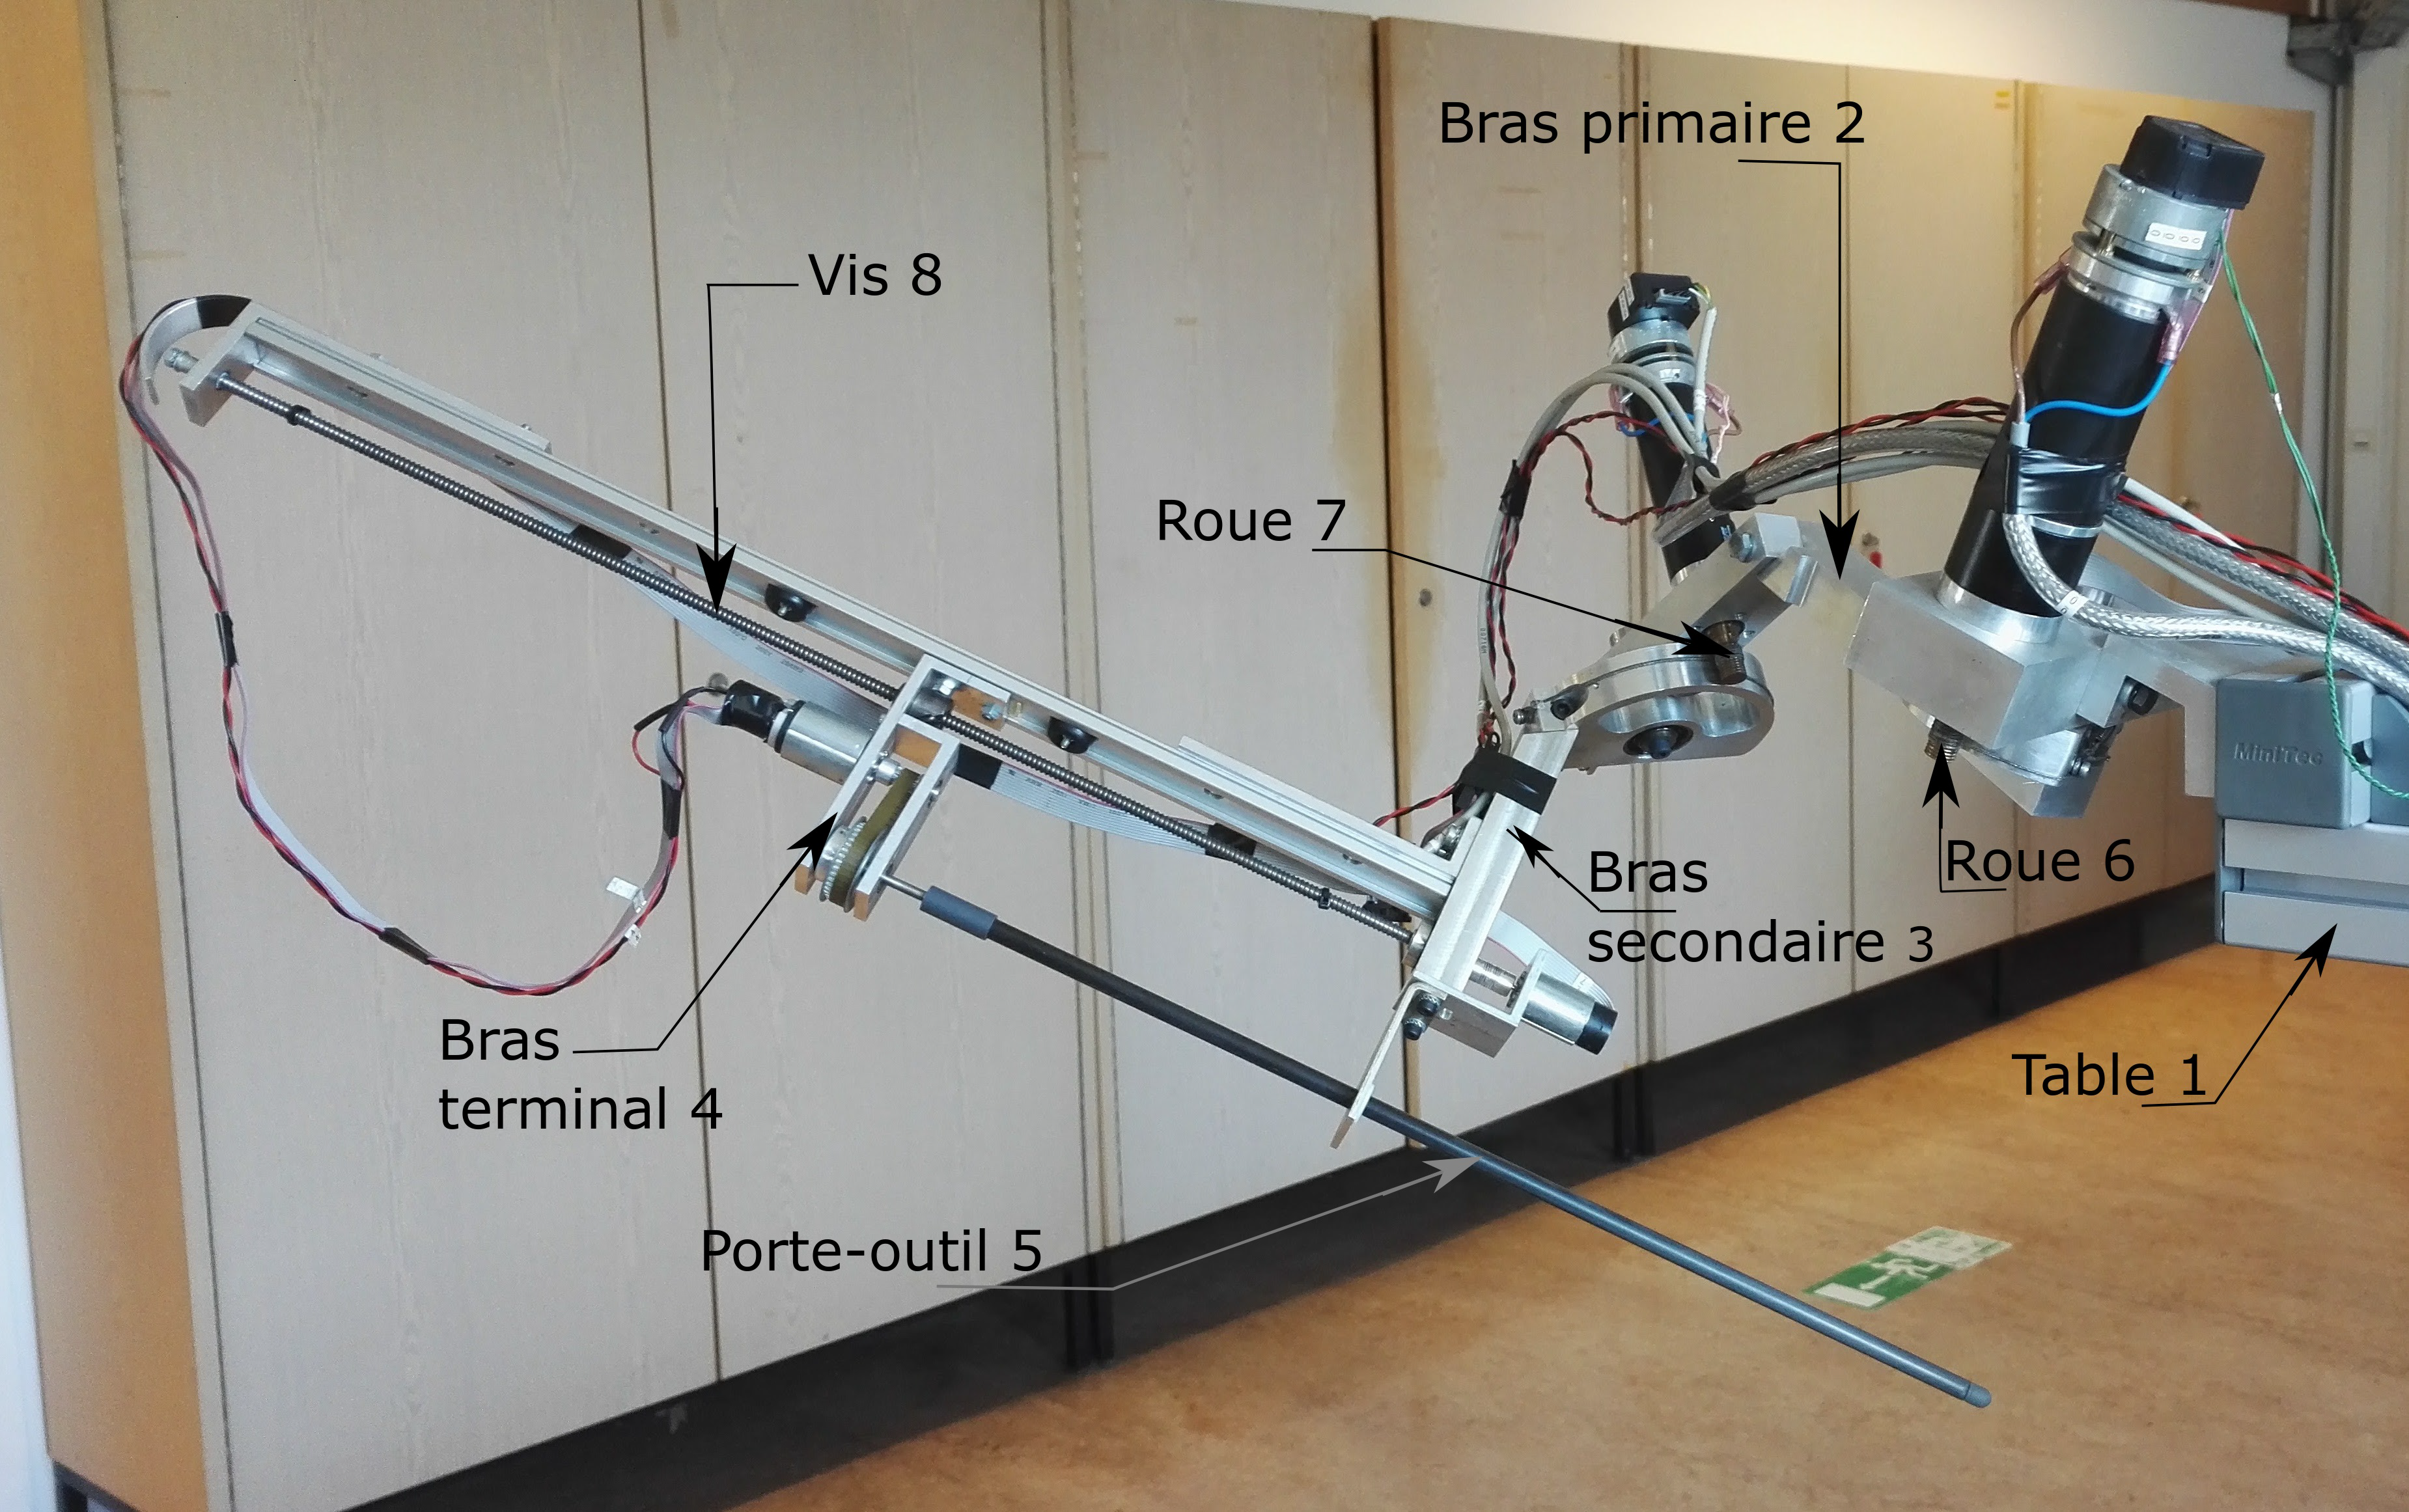
\includegraphics[width=.6\linewidth]{fig_00}
}%figues de la page de garde


\input{pagegarde_info}

\setlength{\columnseprule}{.1pt}

\pagestyle{fancy}
\thispagestyle{plain}

\vspace{4.5cm}


\def\columnseprulecolor{\color{ocre}}
\setlength{\columnseprule}{0.4pt} 

%%%%%%%%%%%%%%%%%%%%%%%

\setcounter{exo}{0}
\vspace{2cm}
%\begin{multicols}{2}

\subsection*{Pour Texmaker}
J'ai vu ça : 


Dans Utilisateur -> Commandes utilisateurs -> Éditer les commandes utilisateurs, choisir
une commande, puis dans Item menu, taper : Pythontex et la commande est (en une seule
ligne) :
\begin{pyverbatim}
pdflatex --shell-escape -synctex=1 -interaction=nonstopmode %.tex
|pythontex %.tex|pdflatex --shell-escape -synctex=1
-interaction=nonstopmode %.tex
\end{pyverbatim}

Pour chez moi, j'utilise un .bat que je t'ai mis dans le dossier.

Sinon, vu qu'il y a souvent des bug je compile a la main.
pdflatex fichier.tex
pythontex fichier.tex
pdflatex fichier.tex


\subsection*{Mise en forme du code avec pyv et pyverbatim}

\subparagraph{}\textit{Donner l'algorithme permettant de calculer l'intégrale d'une fonction sur un intervalle $[a,b]$ en utilisant la méthode des rectangles à droite. Pour cela on implémentera la fonction 
\pyv{ def IntRectDroite(f:function, a:float, b:float, n:int) -> float : }.}

(Les césure de pyv sont pourries :) )
\begin{pyverbatim}
def foo(x):
    print(x)

foo("Pyverbatim n'interprète pas le code")
\end{pyverbatim}

\subsection*{Interprétation du code avec pyc, pyb, py, pycode}

Pyc interprète mais n'affiche rien : \pyc{bar1 ='Coucou'}.

Pyb interprète et affiche le code (et pas le résultat) : \pyb{bar2 ='Salut'; print (bar2);}.

Py affiche le résultat \py{bar1}, \py{bar2}.

Pycode, comme pyc n'affiche rien, mais c'est interprété. 

\begin{pycode}
import numpy as np
import matplotlib.pyplot as plt
plt.plot(np.linspace(0,4),np.sin(np.linspace(0,1)))
plt.savefig('toto.pdf')
\end{pycode}

\includegraphics[width=.4\linewidth]{toto}

\subsection*{Générateur de console avec pyconsole}
\begin{pyconsole}
a=1
b=2
print(a,b)
\end{pyconsole}




%\end{multicols}

\end{document}